

\tikzset{every picture/.style={line width=0.75pt}} %set default line width to 0.75pt        

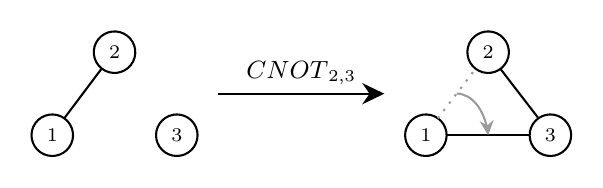
\begin{tikzpicture}[x=0.75pt,y=0.75pt,yscale=-1,xscale=1]
%uncomment if require: \path (0,162); %set diagram left start at 0, and has height of 162

%Shape: Circle [id:dp23417453743827976] 
\draw   (87.86,66.18) .. controls (84.45,70.52) and (78.17,71.28) .. (73.82,67.86) .. controls (69.48,64.45) and (68.72,58.17) .. (72.14,53.82) .. controls (75.55,49.48) and (81.83,48.72) .. (86.18,52.14) .. controls (90.52,55.55) and (91.28,61.83) .. (87.86,66.18) -- cycle ;
%Shape: Circle [id:dp011544140967992389] 
\draw   (41.84,94.21) .. controls (45.04,89.71) and (51.28,88.65) .. (55.79,91.84) .. controls (60.29,95.04) and (61.35,101.28) .. (58.16,105.79) .. controls (54.96,110.29) and (48.72,111.35) .. (44.21,108.16) .. controls (39.71,104.96) and (38.65,98.72) .. (41.84,94.21) -- cycle ;
%Shape: Circle [id:dp416194828283707] 
\draw   (101.66,105.51) .. controls (98.61,100.91) and (99.88,94.7) .. (104.49,91.66) .. controls (109.09,88.61) and (115.3,89.88) .. (118.34,94.49) .. controls (121.39,99.09) and (120.12,105.3) .. (115.51,108.34) .. controls (110.91,111.39) and (104.7,110.12) .. (101.66,105.51) -- cycle ;
%Straight Lines [id:da17802990060125945] 
\draw    (73.82,67.86) -- (55.79,91.84) ;
%Shape: Circle [id:dp026916354896634798] 
\draw   (267.97,66.03) .. controls (264.64,70.44) and (258.37,71.31) .. (253.96,67.97) .. controls (249.56,64.64) and (248.69,58.37) .. (252.02,53.96) .. controls (255.36,49.56) and (261.63,48.69) .. (266.03,52.02) .. controls (270.44,55.36) and (271.31,61.63) .. (267.97,66.03) -- cycle ;
%Shape: Circle [id:dp9684318791918579] 
\draw   (221.84,94.21) .. controls (225.04,89.71) and (231.28,88.65) .. (235.78,91.84) .. controls (240.29,95.04) and (241.35,101.28) .. (238.15,105.78) .. controls (234.96,110.29) and (228.72,111.35) .. (224.21,108.15) .. controls (219.71,104.96) and (218.65,98.72) .. (221.84,94.21) -- cycle ;
%Straight Lines [id:da43300710363321016] 
\draw    (265.93,68.05) -- (284.24,91.82) ;
%Shape: Circle [id:dp3103272610346469] 
\draw   (281.82,105.75) .. controls (278.64,101.24) and (279.73,95) .. (284.24,91.82) .. controls (288.76,88.64) and (295,89.73) .. (298.18,94.24) .. controls (301.36,98.76) and (300.27,105) .. (295.75,108.18) .. controls (291.24,111.36) and (285,110.27) .. (281.82,105.75) -- cycle ;
%Straight Lines [id:da6511414638961373] 
\draw    (130,80) -- (207,80) ;
\draw [shift={(210,80)}, rotate = 180] [fill={rgb, 255:red, 0; green, 0; blue, 0 }  ][line width=0.08]  [draw opacity=0] (10.72,-5.15) -- (0,0) -- (10.72,5.15) -- (7.12,0) -- cycle    ;
%Straight Lines [id:da1905731404703308] 
\draw    (240,100) -- (280,100) ;
%Straight Lines [id:da19331622592606712] 
\draw [color={rgb, 255:red, 155; green, 155; blue, 155 }  ,draw opacity=1 ] [dash pattern={on 0.84pt off 2.51pt}]  (235.78,91.84) -- (253.96,67.97) ;
%Curve Lines [id:da4343842529052825] 
\draw [color={rgb, 255:red, 155; green, 155; blue, 155 }  ,draw opacity=1 ]   (244.87,79.91) .. controls (252.59,80.17) and (257.91,88.06) .. (259.59,97.12) ;
\draw [shift={(260,100)}, rotate = 264.4] [fill={rgb, 255:red, 155; green, 155; blue, 155 }  ,fill opacity=1 ][line width=0.08]  [draw opacity=0] (7.14,-3.43) -- (0,0) -- (7.14,3.43) -- (4.74,0) -- cycle    ;

% Text Node
\draw (50,100) node  [font=\scriptsize]  {$1$};
% Text Node
\draw (80,60) node  [font=\scriptsize]  {$2$};
% Text Node
\draw (110,100) node  [font=\scriptsize]  {$3$};
% Text Node
\draw (230,100) node  [font=\scriptsize]  {$1$};
% Text Node
\draw (260,60) node  [font=\scriptsize]  {$2$};
% Text Node
\draw (290,100) node  [font=\scriptsize]  {$3$};
% Text Node
\draw (170,77) node [anchor=south] [inner sep=0.75pt]  [font=\small] [align=left] {$\displaystyle \text{CNOT}_{2,3}$};


\end{tikzpicture}